\documentclass{article}

\usepackage{float}
\usepackage{amsmath}
\usepackage{graphicx}
\usepackage{booktabs}

\title{Assignment of ET 4389}
\author{Volker Strobel}
\date{\today}

\begin{document}
\maketitle
\subsection*{1)}
$G$ is the network described in \texttt{7.txt}.

\begin{itemize}
  \item Number of nodes $N$: $379$ 
  \item Number of links $L$: $914$
  \item Link density $p$: $0.013$
  \item Average degree $E[D]$: $4.82$
  \item Degree variance $Var[D]$: $15.46$
\end{itemize}

\begin{figure}[H]
  \centering
  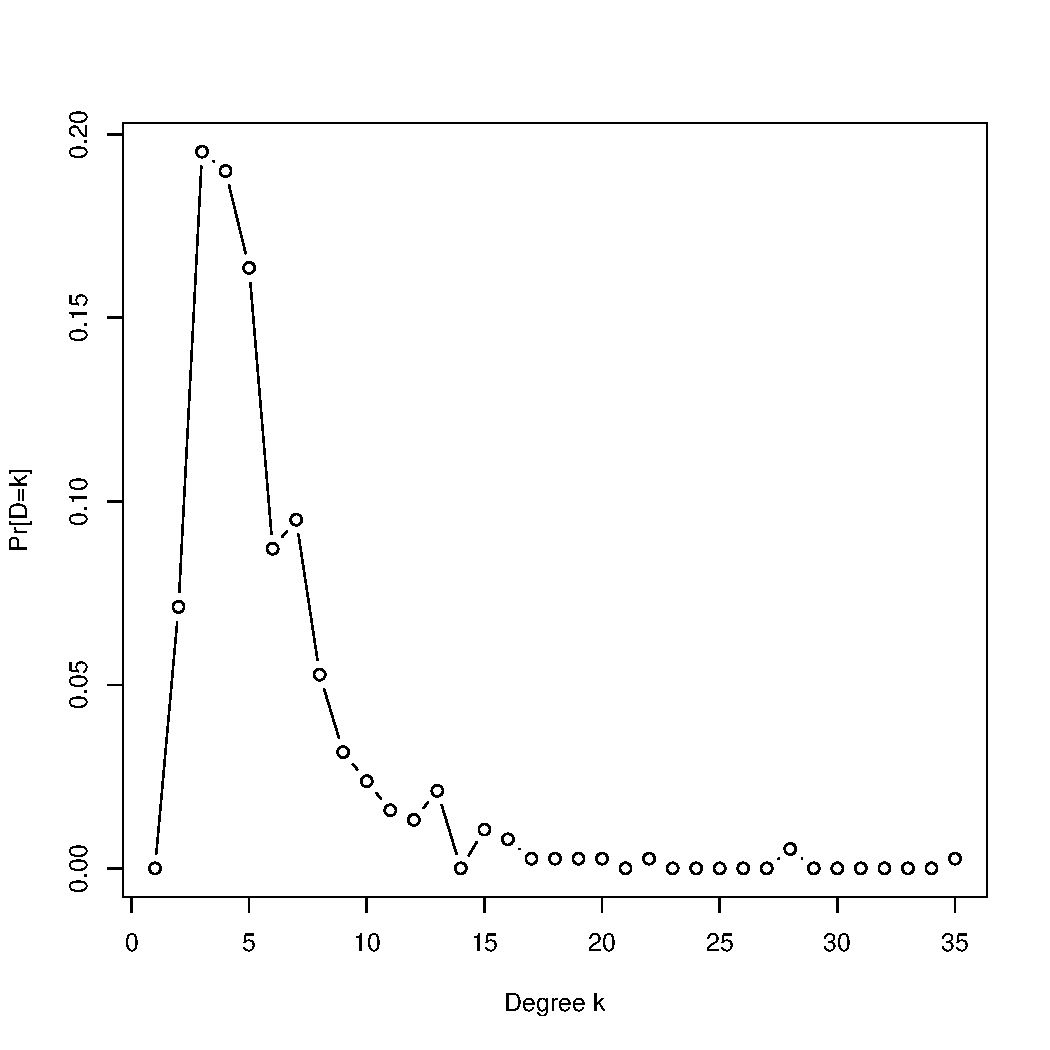
\includegraphics[width=0.7\textwidth]{degree_distribution}
  \caption{Degree distribution of Graph $G$}
\end{figure}

\subsection*{2)}

\begin{itemize}
\item Degree correlation (assortativity) $\rho_D$: $-0.30$
\end{itemize}
\textbf{Physical meaning}:\\
Assortativity $\sim$ \emph{Birds of a feather flock together.}\\
Disassortativity $\sim$ \emph{Opposites attract.}

\vspace*{0.5em}
\noindent Networks, in which nodes with a high degree are likely
connected to other high-degree nodes are \emph{assortative}; networks
in which nodes with a low degree are likely connected to high-degree
nodes are \emph{disassortative}.

\subsection*{3)}

\begin{itemize}
  \item Clustering coefficient: $0.17$
\end{itemize}

\subsection*{4)}

\begin{itemize}
  \item Average hopcount $E[H]$: $3.75$
  \item Diameter $H_{max}$: $7$
\end{itemize}

\subsection*{5)}
\begin{itemize}
  \item Largest eigenvalue (spectral radius) $\lambda_1$: $7.44$
\end{itemize}
\subsection*{6)}

\begin{itemize}
\item Second smallest eigenvalue (algebraic connectivity) of the
  Laplacian matrix $\mu_{N-1}$: $0.40$
\end{itemize}

\subsection*{7)}
Now, we consider the network $G_N$, described in \texttt{NetScience.txt}.

\begin{itemize}
\item Number of nodes $N$: $379$
\item Number of links $L$: $914$
\item Link density $p$: $0.013$
\item Average degree $E[D]$: $4.82$
\item Degree variance $Var[D]$: $15.46$
\item Clustering coefficient $C$: $0.80$
\item Assortativity $\rho_D$: $-0.08$
\item Average hopcount $E[H]$: $6.04$
\item Spectral radius $\lambda_1$: $10.38$
\item Algebraic connectivity $\mu_{N-1}$: $0.015$
\item Diameter $H_{max}$: $17$
\end{itemize}

\subsection*{8)}

I am discussing the metrics in the sense of ``which network may allow
information to propagte to a larger fraction of the network''.
\vspace*{0.5em}

\noindent\emph{Clustering coefficient $C$}. The clustering coefficient $C$
states how densely the neighbors of a node are connected, that is, are
my friends also friends with eeach other. Here, $G_N$ performs much
better ($C(G) = 0.17 < C(G_N) = 0.80$), and is therefore better
suited, since information can reach me on several channels, and makes
the network more robust.

\vspace*{0.5em}
\noindent\emph{Average degree E[H]}. The average degree states the amount of
neighbors of a node in a graph, in a communication network, to how
many entities a message could be directly sent. Since both networks
$G$ and $G_N$ have the same average degree, none of them performs
better here.

\vspace*{0.5em}
\noindent\emph{Diameter $H_{max}$}. The diameter of the communication network
states how many edges a message needs to pass between two nodes in the
worst case. Since a smaller $H_{max}$ means faster communication in
the worst case, $G$ performs better ($H_{max}(G) = 7 < H_{max}(G_N) =
17$).

\vspace*{0.5em}
\noindent\emph{Spectral radius $\lambda_1$}. The spectral radius is important
for dynamic processes in networks, for example, if, and how fast, a
message might go ``viral'' but also how fast a virus might affect the
network. The larger $lambda_1$, the lower the epidemic threshold
$\tau_c$. Regarding security, a higher $lambda_1$ is better,
therefore, $G$ performs better ($\lambda_1(G) = 7.44 < \lambda_1(G_N)
= 10.38$).

\vspace*{0.5em}
\noindent\emph{Algebraic connectivity $\mu_{N-1}$}. This metric states how well connected a graph is
and, if the value is greater than zero, that the graph consits of one
connected component. Since $G$ has the higher connectivtity, it
performs better ($\mu_{N-1}(G) = 0.40 > \mu_{N-1}(G_N) = 0.015$).

\vspace*{0.5em}
\noindent All in all, I would recommend design $G$, and is better suited to
convey information across the network.

\subsection*{9)}

\begin{figure}[H]
  \centering
  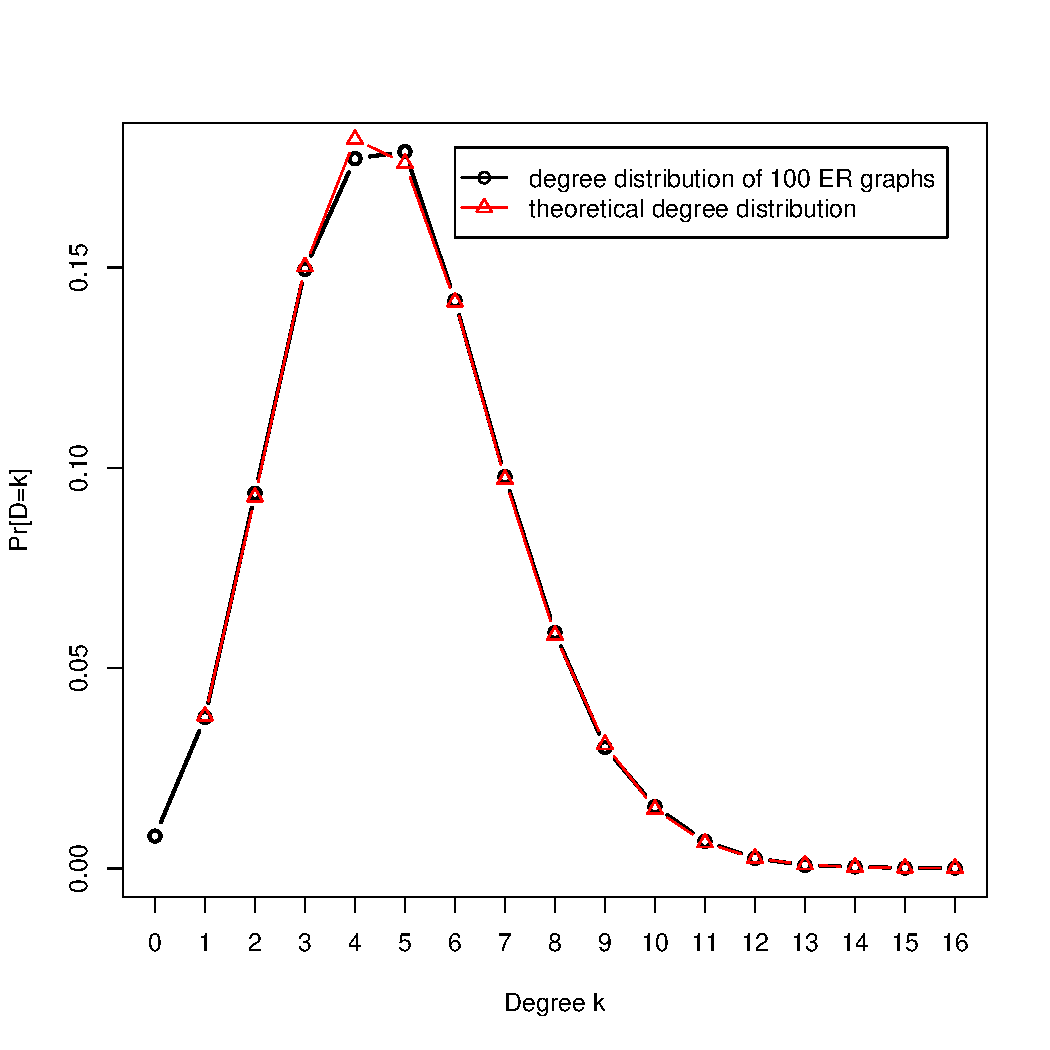
\includegraphics[width=0.9\textwidth]{er_degree_distribution}
  \caption{Comparison of the degree distribution of 100 ER instances
    and the theoretical degree distribution, where $Pr[D=k] =
    \binom{N-1}{k}p^k(1-p)^{N-1-k}=\binom{378}{k}0.013^k\cdot0.987^{378-k}$.}
\end{figure}


\subsection*{10)}
Average of the metrics over the 100 ER random networks:
\begin{itemize}
 \item Number of nodes $N$: 379
 \item Number of links $L$: 914.33
 \item Link density $p$: 0.012764
 \item Average degree $E[D]$: 4.824960
 \item Degree variance $Var[D]$: 4.774007
 \item Clustering coefficient: 0.012574
 \item Assortativity: -0.003513
 \item Average hopcount $E[H]$: 3.928829
 \item Spectral radius $\lambda_1$: 6.006430
 \item Algebraic connectivity $\mu_{N-1}$: 0.025853
 \item Diameter $H_{max}$: 7.980000
\end{itemize}

\subsection*{11)}


Now, we have a feeling of which network is better suited for
information propagation.  However, there are still limitations: for
example the speed of information propagation. We know, how many nodes
are infected in the $E[n_{R_\infty}]$ state, but not how fast that
occured.

\begin{table}[H]
  \centering
  \begin{tabular}{r|rrr}
    \toprule
Metric      & $G$   & $G_N$ & 100 ER \\
\midrule
$N$         & 379   & 379   & 379    \\
$L$         & 914   & 914   & 914.33 \\
$p$         & 0.013 & 0.013 & 0.013  \\
$E[D]$      & 4.82  & 4.82  & 4.82   \\
$Var[D]$    & 15.46 & 15.46 & 4.77   \\
$C$         & 0.17  & 0.80  & 0.01  \\
$\rho_D$    & -0.30 & -0.08 & 0.00   \\
$E[H]$      & 3.75  & 6.04  & 3.93   \\
$\lambda_1$ & 7.44  & 10.38 & 6.01   \\
$\mu_{N-1}$ & 0.40  & 0.015 & 0.026  \\
$H_{max}$   & 7     & 17    & 7.98   \\
\bottomrule
  \end{tabular}
  \caption{Comparison of all metrics}
\end{table}

\end{document}
